\documentclass[12pt]{article}

\usepackage{times}
\usepackage{graphicx}
\usepackage{amsmath}
\usepackage{url}

\setlength{\textwidth}{6.5in}
\setlength{\textheight}{8.9in}
\setlength{\oddsidemargin}{0.0in}
\setlength{\topmargin}{0.05in}
\setlength{\headheight}{-0.05in}
\setlength{\headsep}{0.0in}

\newcommand{\indep}{\perp\!\!\!\perp}

\begin{document}

\begin{center}
{\bf CS 6300} \hfill {\large\bf HW8: Bayes Nets II \hfill Due April 11, 2017}
\end{center}

\noindent
Please use the \LaTeX\ template to produce your writeups. See the
Homework Assignments page on the class website for details.  Hand in
at: \url{https://webhandin.eng.utah.edu/index.php}.

\section{Variable Elimination}

Perform variable elimination on the network below to figure out $P(C)$
given $F=f$ and $D= \sim d$. Show your work and list all of the
intermediate factors formed. Assume we eliminate the variables in the
following order: F, E, D, B, A.

\begin{center}
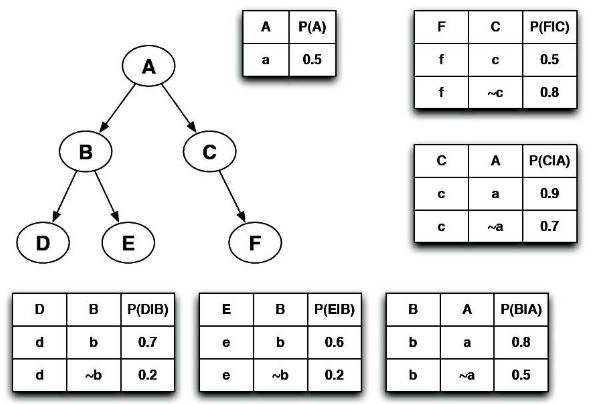
\includegraphics[width=5in]{prob1.png}
\end{center}

To elimate the variables, we can sum over them all individually. This gives the equation

\begin{align*}
  P(C) &= P(f|C)\sum_{A}P(C|A)P(A)\sum_{B}P(B|A)P(\sim d|B)\sum_{E}P(E|B)
  \intertext{In using this, we can caluclate the values for $c$ and $\sim c$, giving}
  P(c, \sim d, f) &= 0.5(0.9\cdot 0.5 + 0.7 \cdot 0.5)(0.8 \cdot 0.3 + 0.5 \cdot 0.8)(0.8)\\
       &= 0.2048\\
 P(\sim c, \sim d, f) &= 0.8(0.1\cdot 0.5 + 0.3 \cdot 0.5)(0.8 \cdot 0.3 + 0.5 \cdot 0.8)(0.8)\\
       &= 0.0819
\intertext{Now, solving for $P(c|\sim d, f)$ and $P(\sim c|\sim d, f)$ gives}
P(c|\sim d, f) &= \frac{P(c,f,\sim d)}{\sum_{C}P(c,f,\sim d)}\\
               &= \frac{0.2048}{0.2048 + 0.0819} = 0.7143\\
P(\sim c| \sim d, f) &= \frac{P(\sim c,f,\sim d)}{\sum_{C}P(c,f,\sim d)}\\
&= \frac{0.08192}{0.2048 + 0.0819} = 0.2857\\
\end{align*}

\clearpage

\section{Sampling}

Consider the Bayes net below with corresponding CPTs.  

\begin{enumerate}

\item Generate 2 samples using the following random numbers.  The
  order for the random numbers is ABCD.

\begin{center}
\begin{tabular}{|c|c|c|c|c|c|c|c|c|c|} \hline
0.31 & 0.58 & 0.04 & 0.94 & 0.67 & 0.49 & 0.37 & 0.42 & \ldots \\ \hline
\end{tabular}
\end{center}

\begin{center}
\begin{tabular}{cc}
\begin{tabular}{cccc}
\begin{tabular}{|c|c|} \hline
A  & P(A) \\ \hline
+a & 0.8  \\ \hline
-a & 0.2  \\ \hline
\end{tabular} & 
\begin{tabular}{|r|r|r|} \hline
A  & B  & $P(B|A)$ \\ \hline
+a & +b & 0.8  \\ \hline
+a & -b & 0.2  \\ \hline
-a & +b & 0.5  \\ \hline
-a & -b & 0.5  \\ \hline
\end{tabular} \\[.4in]
\begin{tabular}{|r|r|r|} \hline
A  & C  & $P(C|A)$ \\ \hline
+a & +c & 0.7  \\ \hline
+a & -c & 0.3  \\ \hline
-a & +c & 0.1  \\ \hline
-a & -c & 0.9  \\ \hline
\end{tabular} &
\begin{tabular}{|r|r|r|r|} \hline
B  & C  & D  & $P(D|B,C)$ \\ \hline
+b & +c & +d & 0.3      \\ \hline
+b & +c & -d & 0.7      \\ \hline
+b & -c & +d & 0.1      \\ \hline
+b & -c & -d & 0.9      \\ \hline
-b & +c & +d & 0.2      \\ \hline
-b & +c & -d & 0.8      \\ \hline
-b & -c & +d & 0.9      \\ \hline
-b & -c & -d & 0.1      \\ \hline
\end{tabular}
\end{tabular} & 
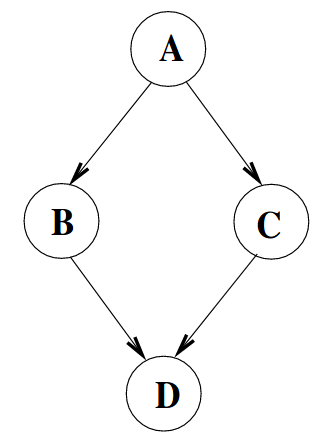
\includegraphics[height=2in]{prob2.png}
\end{tabular}
\end{center}

\item Given the samples below, answer the subsequent queries.

\begin{flushleft}
\begin{tabular}{rrrrr} 
+a & -b & -c & -d  \\
-a & +b & +c & -d  \\
+a & -b & +c & -d  \\
+a & +b & -c & -d  \\
+a & -b & +c & +d  \\
-a & -b & -c & +d  \\
-a & -b & -c & -d  \\
+a & +b & +c & -d  \\
-a & +b & -c & -d  \\
+a & +b & -c & +d  \\
\end{tabular}
\end{flushleft}

\begin{enumerate}

  \item $P(+d) = 3/10$

  \item $P(+a,-b) = 2/10$

  \item $P(-a,-b,-c,-d) = 1/10$

  \item $P(-c | -d) = 4/7$

  \item $P(+d | -a, -b) = 1/2$

\end{enumerate}

\item Consider the query $P(-d|-a,-b)$.  Using the same random numbers
  as before, generate samples and their weights using likelihood
  weighting.

\begin{center}
\begin{tabular}{|c|c|c|c|c|c|c|c|c|c|} \hline
0.31 & 0.58 & 0.04 & 0.94 & 0.67 & 0.49 & 0.37 & 0.42 & \ldots \\ \hline
\end{tabular}
\end{center}

\item Given the weighted samples below, answer the subsequent queries.

\begin{flushleft}
\begin{tabular}{rrrrr} 
+a & -b & -c & -d & 0.3 \\
-a & +b & +c & -d & 0.4 \\
+a & -b & +c & -d & 0.1 \\
+a & +b & -c & -d & 0.3 \\
+a & -b & +c & +d & 0.4 \\
-a & -b & -c & +d & 0.1 \\
-a & -b & -c & -d & 0.2 \\
+a & +b & +c & -d & 0.5 \\
-a & +b & -c & -d & 0.7 \\
+a & +b & -c & +d & 0.8 \\
\end{tabular}
\end{flushleft}

\begin{enumerate}

  \item $P(+d)$

  \item $P(+a,-b)$

  \item $P(-a,-b,-c,-d)$

  \item $P(-c | -d)$

  \item $P(+d | -a, -b)$

\end{enumerate}

\end{enumerate}

\end{document}


